\section{Part of Speech (POS) Tagging with Conditional Random Field (CRF)}
\subsection*{Description}
\emph{Task} --- 
\begin{itemize}
    \item Tag parts of speech, e.g., adverb, verb, noun, etc.
\end{itemize}

{\color{black}\hrule height 0.001mm}

\subsection*{Formulation}
\begin{itemize}
    \item Input: Sequence of words $w$ of length $N$
    \item Output: Sequence of tags $t \in T$ with $t_0 = BOS$ and $t_N = EOS$
    \item Can represented as \emph{trellis}:
    \begin{itemize}
        \item DAG, where nodes are divided into vertical slices and each slice is associated with a timestamp
        \item Each node corresponds to a distinct state
        \item Each arrow represents a transition to a new state in the next slice
    \end{itemize}
\end{itemize}

{\color{lightgray}\hrule height 0.001mm}

\emph{Point of departure} --- 
\begin{itemize}
    \item Log-linear model:
    $
    p(t \mid w) = \frac{\exp(\textrm{score}(t, w))}{Z} = \frac{\exp(\textrm{score}(t, w))}{\sum_{t'} \exp(\textrm{score}(t', w))}
    $
    \item Challenge: Naively computing $Z$ would take exponential time $\mathcal{O}(|T|^N)$
    \item Solution: Consider a scoring function that is additively decomposable over tag bigrams:
    $
    \textrm{score}(t, w) = \sum_{n=1}^N \textrm{score}(\langle t_{n-1}, t_n \rangle, w)
    $
    \item Then, we have:
    $
    p(t \mid w) = \frac{\exp( \sum_{n=1}^N \textrm{score}(\langle t_{n-1}, t_n \rangle, w) )}{\sum_{t'} \exp( \sum_{n=1}^N \textrm{score}(\langle t_{n-1}', t_n' \rangle, w) )}
    $
    \item If we take the denominator:
    \begin{itemize}
        \item $
        \sum_{t_1:t_N} \exp( \sum_{n=1}^N \dots ) = \sum_{t_1:t_N} \prod_{n=1}^N \exp(\dots) = \sum_{t_1:t_{N-1}} \sum_{t_N} \prod_{n=1}^N \exp(\dots)
        $ since last tag $t_N$ only depends on $t_{N-1}$
        \item $ = \sum_{t_1:t_{N-1}} \prod_{n=1}^{N-1} \exp(\dots) $\\$\sum_{t_N} \prod_{n=N}^{N} \exp(\textrm{score}(\langle t_{n-1}, t_n \rangle, w) ) 
        $ based on distributivity of $\otimes$ over $\oplus$
        \item $ = \sum_{t_1:t_{N-1}} \prod_{n=1}^{N-1} \exp(\dots) $\\$\sum_{t_N} \exp(\textrm{score}(\langle t_{N-1}, t_N \rangle, w) ) 
        $
        \item $ = \sum_{t_1} [ \exp(\textrm{score}(\langle t_0, t_1 \rangle, w) ) \times \sum_{t_2} [ \exp(\dots) \times \dots \times \sum_{t_N} \exp(\textrm{score}(\langle t_{N-1}, t_N \rangle, w) )]]
        $
    \end{itemize}
    \item We've moved from an exponential number of terms to a linear number of terms
    \item We go from having a score for each path in the trellis to a score for each edge
\end{itemize}

{\color{lightgray}\hrule height 0.001mm}

\emph{Backward algorithm} --- 
\begin{itemize}
    \item Algorithm for computing $Z$
    \begin{enumerate}
        \item For $t_{N-1}$ (all tags):
        $
        \beta(w, t_{N-1}) \gets \exp(\textrm{score}(\langle t_{N-1}, \textrm{EOS} \rangle, w))
        $
        \begin{itemize}
            \item Handles scores of edges incoming to EOS
            \item $\beta$ is memoized
        \end{itemize}
        \item For $n \in N-2, \dots, 1$:\\
        For $t_n \in T$ (all tags):
        $
        \beta(w, t_n) \gets \sum_{t_{n+1}} \exp(\textrm{score}(\langle t_n, t_{n+1} \rangle, w)) \times \beta(w, t_{n+1})
        $
        \begin{itemize}
            \item Handles scores over normal edges
            \item $\beta$ is memoized
        \end{itemize}
        \item 
        $
        \beta(w, t_0) \gets \sum_{t_1} \exp(\textrm{score}(\langle \textrm{BOS}, t_1 \rangle, w)) \times \beta(w, t_1)
        $
        \begin{itemize}
            \item Handles scores of edges outgoing from BOS
        \end{itemize}
        \item Return $\beta(w, t_0)$
    \end{enumerate}
    \item $\beta(w, t_n)$ are \emph{backward variables} that contain the sum of the scores of all paths starting at EOS and ending at tag $t_n$
    \item Therefore:
    $
    \textrm{denominator} = \beta(w, t_0) = \beta(w, \textrm{BOS})
    $
    \item Complexity:
    \begin{itemize}
        \item Time complexity: 
        \begin{itemize}
            \item For scoring function over tag bigrams: $\mathcal{O}(N |T|^2)$, given that we compute $|T| N$ backward variables and for each of them, compute the sum over $|T|$ successor tags
            \item For scoring function over tag trigrams: $\mathcal{O}(N |T|^3)$
            \item For scoring function over tag N-grams of order $n$: $\mathcal{O}(N |T|^{n})$
        \end{itemize}
        \item Space complexity: $\mathcal{O}(N|T|)$, since we have to keep $|T| N$ backward variables in memory
    \end{itemize}
    \item Alternatively, the same can be achieved with a \emph{forward algorithm}
    \begin{itemize}
        \item Starting from BOS $t_0$ and going forward towards EOS $t_N$
        \item Instead of looking at $t_{n+1}$ we look at $t_{n-1}$
    \end{itemize}
    \item In addition to probabilities, we can compute entropy of the CRF using the expectation semiring:
    \begin{itemize}
        \item Instead of $\omega = \exp(\textrm{score}(\langle t_{n-1}, t_n \rangle, w))$, we do:
        $
        \omega = \langle \omega, -\omega \log(\omega) \rangle
        $
        \item Running the backward algorithm with these weights and in the expectation semiring, we can additionally compute unnormalized entropy $H_u = - \sum_t \exp(\textrm{score}(t, w)) \times \textrm{score}(t, w)$ in the same runtime complexity:
        \begin{itemize}
            \item We aim to show that the backward algorithm computes $\langle Z, H_u\rangle$
            \item In the base case, $\langle Z, H_u\rangle = \langle \omega, -\omega \log(\omega) \rangle$
            \item Let's call the adjusted backward variables $\beta'$, instead of $\beta$
            \item $
            \beta'(w, t_n)  \gets \bigoplus_t 
            \langle \omega(t_n, t_{n+1}), -\omega(t_n, t_{n+1}) \log(\omega(t_n, t_{n+1})) \rangle \otimes \beta'(w, t_{n+1})
            $
            \item Based on the definition of $\otimes$ under the expectation semiring, this is: $
            \beta'(w, t_n)  \gets \bigoplus_t 
            \langle Z_{n-1} \times \omega(t_n, t_{n+1}), Z_{n-1} \times -\omega(t_n, t_{n+1}) \log(\omega(t_n, t_{n+1})) + H_{u,n-1} \times \omega(t_n, t_{n+1}) \rangle = 
            \langle Z_{n-1} \times \omega(t_n, t_{n+1}), [Z_{n-1} \times -\log(\omega(t_n, t_{n+1})) + H_{u,n-1}] \times \omega(t_n, t_{n+1}) \rangle
            $
            \item Then:
            \begin{itemize}
                \item $Z_{n-1} = \sum_t \prod_{i=1}^{n-1} \omega(t_n, t_{n+1}) = \sum_t \exp(\textrm{score}(t, w))$
                \item $H_{u,n-1} = \sum_t [ \prod_{i=1}^{n-1} \omega(t_n, t_{n+1}) ][ \sum_{i=1}^{n-1} -\log(\omega(t_n, t_{n+1})) ] = -\sum_t [ \prod_{i=1}^{n-1} \omega(t_n, t_{n+1}) ][ \log(\prod_{i=1}^{n-1} \omega(t_n, t_{n+1})) ] = - \sum_t \exp(\textrm{score}(t, w)) \times \textrm{score}(t, w)$
            \end{itemize}
        \end{itemize}
        \item We can then compute the normalized entropy $H_n$:
        \begin{itemize}
            \item $H_n = -\sum_t p(t) \log(p(t))$
            \item If we substitute $p(t) = \frac{1}{Z} \exp(\textrm{score}(t, w))$, we get: $H_n = -\sum_t \frac{1}{Z} \exp(\textrm{score}(t, w)) \log(\frac{1}{Z} \exp(\textrm{score}(t, w)))$
            \item We can develop to:
            $H_n = -\sum_t \frac{1}{Z} \exp(\textrm{score}(t, w)) (\textrm{score}(t, w) - \log(Z)) = -\sum_t \frac{1}{Z} \exp(\textrm{score}(t, w))\textrm{score}(t, w) - \frac{1}{Z} \exp(\textrm{score}(t, w)) \log(Z) = \frac{1}{Z} \sum_t -[ \exp(\textrm{score}(t, w))\textrm{score}(t, w)] + \log(Z)\sum_t[\frac{1}{Z} \exp(\textrm{score}(t, w))] = \frac{1}{Z} \sum_t -[ \exp(\textrm{score}(t, w))\textrm{score}(t, w)] + \log(Z) \times 1 = Z^{-1} H_u + \log(Z)$
        \end{itemize}
    \end{itemize}
\end{itemize}

{\color{lightgray}\hrule height 0.001mm}

\emph{Viterbi algorithm} --- 
\begin{itemize}
    \item Algorithm for computing the score of the best tag sequence $t^*$ and recovering the sequence itself
    \item For this, we can ignore the denominator: $
    p(t \mid w) \propto \exp(\textrm{score}(t, w))
    $
    \begin{enumerate}
        \item For $t_{N-1}$ (all tags):
        \begin{itemize}
            \item $v(w, t_{N-1}) \gets \exp(\textrm{score}(\langle t_{N-1}, \textrm{EOS} \rangle, w))$
            \item $
            b(t_{N-1}) \gets \textrm{EOS}$ since $t_N$ can only be EOS
        \end{itemize}
        \item For $n \in N-2, \dots, 1$:\\
        For $t_n \in T$ (all tags):
        \begin{itemize}
            \item
            $
            v(w, t_n) \gets \max_{t_{n+1}} [ \exp(\textrm{score}(\langle t_n, t_{n+1} \rangle, w)) \times v(w, t_{n+1}) ]
            $ for each tag $t_n$, stores the score of the next best tag $t_{n+1}$ 
            \item $
            b(t_n) \gets argmax_{t_{n+1}} [ \exp(\textrm{score}(\langle t_n, t_{n+1} \rangle, w)) \times v(w, t_{n+1}) ]
            $ for each tag $t_n$, stores the tag $t_{n+1}$ that gave the best score
        \end{itemize}
        \item Finally:
        \begin{itemize}
            \item $
            v(w, t_0) \gets \max_{t_1} [  \exp(\textrm{score}(\langle t_0, t_1 \rangle, w)) \times v(w, t_1)]
            $
            \item $
            b(t_0) \gets argmax_{t_1} [  \exp(\textrm{score}(\langle t_0, t_1 \rangle, w)) \times v(w, t_1)]
            $
        \end{itemize}
        \item For $n = 1, \dots, N$: Recover the best sequence using backpointers, by always plugging in next $t$
        $
        t_n \gets b(t_{n-1})
        $
        \begin{itemize}
            \item $t_1 = b(\textrm{BOS})$
            \item $t_2 = b(t_1)$
            \item $...$
        \end{itemize}
        \item Return $t_{1:N}$ and $v(w, t_0)$
    \end{enumerate}
    \item $b(t_n)$ are \emph{backpointers} that point to the $t_{n+1}$ tag in $t^*$
    \item $v(w, t_n)$ are \emph{Viterbi variables} that contain the score of $t^*$ starting at EOS and ending with tag $t_n$ 
    \item Complexity:
    \begin{itemize}
        \item For backpointers: $\mathcal{O}(N)$
        \item For scoring function over tag N-grams of order $n$: $\mathcal{O}(N |T|^n)$ 
        \item For higher-order N-grams, we apply restriction that transitions must be valid (e.g. in $t_1 \to t_2, t_3 \to t_4$ $t_2$ must equal $t3$)
    \end{itemize}
    \item Alternatively, the same can be achieved with a \emph{forward Viterbi algorithm}
    \begin{itemize}
        \item Starting from BOS $t_0$ and going forward towards EOS $t_N$
        \item Instead of looking at $t_{n+1}$ we look at $t_{n-1}$
        \item Backpointers point to the $t_{n-1}$ tag in $t^*$, i.e. $t_{n-1} \gets b(t_n)$, starting with $t_{N-1} \gets b(\textrm{EOS}), t_{N-2} \gets b(t_{N-1}),...$
    \end{itemize}
\end{itemize}

{\color{lightgray}\hrule height 0.001mm}

\emph{Dijkstra’s algorithm} --- 
\begin{itemize}
    \item Alternative to the Viterbi algorithm:
    \begin{itemize}
        \item First complete tagging popped from the queue is the score for the best tagging, same as what Viterbi computes
        \item If we keep running Dijkstra’s algorithm until queue is empty (i.e. if we don't leverage early stopping), Dijkstra’s algorithm computes the same values $\gamma$ as Viterbi
    \end{itemize}
    \item Runs over time step - tag nodes $\langle n, t \rangle$
    \item Uses \emph{Popped} to keep track of nodes $\langle n, t \rangle$ that have been processed
    \item Uses \emph{PriorityQueue}:
    \begin{itemize}
        \item Contains node : score pairs $\langle\langle n, t \rangle, \textrm{score}\rangle$
        \item Returns pair with highest score first, regardless of time step or tag, thus, does not necessarily progress over nodes sequentially by time step, but progresses over nodes by descending score
        \item If there is no score yet for key $\langle n, t \rangle$ in queue, it's inserted
        \item If there is already a score for key $\langle n, t \rangle$ in queue, the higher score is retained: $\max_{\textrm{score}} \textrm{score}$
    \end{itemize}
    \item Uses table $\gamma$ to store the best score for each node $\langle n, t \rangle$: $\gamma[n, t] = \textrm{score}$
    \item Algorithm:
    \begin{enumerate}
        \item Initialize:
        \begin{itemize}
            \item Popped $\gets \{ \}$
            \item Queue $\gets$ $\textrm{Priority Queue}()$
            \item $\gamma \gets -\infty$
        \end{itemize}
        \item Push $\langle\langle 0, \textrm{BOS} \rangle, 0\rangle$ to queue
        \item While $|\textrm{queue}| > 0$:
        \begin{enumerate}
            \item Pop $\langle \langle n, t \rangle, \textrm{score} \rangle$ from queue, add $\langle \langle n, t \rangle, \textrm{score} \rangle$ to popped, 
            $
            \gamma[n, t] \gets \textrm{score}
            $
            \item If $n = |w|$ or stop early: Return score    
            \item If $n < |w|$:\\
            For $t' \in T$:\\
            If $\langle n+1, t' \rangle$ is not in popped:
            Push
            $
            \langle \langle n+1, t' \rangle, \textrm{score}(t, t', w) + \gamma[n, t] \rangle
            $
            to queue
        \end{enumerate}
        \item Return $\gamma$
    \end{enumerate}
    \item Complexity:
    \begin{itemize}
        \item For scoring function over tag bigrams: $\mathcal{O}(N |T|^2 \log(N |T|))$, where $\log(N |T|)$ stems from push and update operations on the queue
        \item Dijkstra's is generally slower than Viterbi, unless we leverage early stopping conditions
    \end{itemize}
    \item Dijkstra's as an alternative to Viterbi requires a semiring which guarantees:
    \begin{itemize}
        \item Idempotence of $\oplus$ such that algorithm progresses towards the optimal path without revisiting nodes
        \item Commutative and associative property of $\oplus$ such that score accumulation always yields same result, even if the nodes are processed in a different order
        \item $\mathbb{R}_{\leq0}$ since scores are log-probabilities, which are always non-positive, since probabilities are in $[0,1]$
    \end{itemize}
    \item Dijkstra's could also be used as an alternative to the backward algorithm with a different semiring
    \hl{TBA}
\end{itemize}

{\color{lightgray}\hrule height 0.001mm}

\emph{Generalized algorithm} --- 
\begin{itemize}
    \item A more general formulation of backward, Viterbi, and Dijkstra's algorithms using semirings
    \item Backward algorithm: Uses inside semiring
    \item Viterbi algorithm: Uses Viterbi semiring
    \item Challenge with this original formulation: Multiplying probabilities for long sequences may cause numbers to go to $0$, leading to numerical underflow
    \item Solution: Revert to log-sum-exp semiring (backward algorithm) resp. arctic semiring (Viterbi algorithm)
    \item Dijkstra's algorithm: Uses arctic semiring
\end{itemize}

{\color{lightgray}\hrule height 0.001mm}

\emph{Scoring functions} --- 
\begin{itemize}
    \item So far, we only imposed the requirement that the scoring function is additively decomposable, but we have not specified it further
    \item \emph{Hidden Markov Model}:
    $
    \textrm{score}(\langle t_{n-1}, t_n \rangle,w) = \textrm{transition}(t_{n-1}, t_n) + \textrm{emission}(t_n, w_n) =
    $ transition probability (tag-tag pairs) $+$ emission probability (word-tag pairs) except for $t_N =$ EOS, where we have no emission probability: $
    \textrm{score}(\langle t_{N-1}, t_N \rangle,w) = \textrm{transition}(t_{N-1}, t_N) + 0
    $
    \item A more complex example of scoring functions is a neural network with inputs $\langle t_{n-1}, t_n \rangle$ and $w$
    \item E.g. for the sentence 'The girl drinks':
    \begin{itemize}
        \item $\textrm{score}(w = \textrm{The girl drinks}, t = \langle D, N, V \rangle) = \sum_{n=1}^{N} \textrm{score}(\langle t_{n-1}, t_n \rangle, w)$
        \item $= \textrm{score}(\langle \textrm{BOS}, D \rangle, w) + \textrm{score}(\langle D, N \rangle, w) + \textrm{score}(\langle N, V \rangle, w) + \textrm{score}(\langle V, \textrm{EOS} \rangle, w)$
        \item Combination of emission and transition features: $(w_1 = \textrm{The}, y_1 = D) + (y_1 = D, y_0 = \textrm{BOS}) + (w_2 = \textrm{girl}, y_2 = N) + (y_2 = N, y_1 = D) + (w_3 = \textrm{drinks}, y_3 = V) + (y_3 = V, y_2 = N) + (y_4 = \textrm{EOS}, y_3 = V)$
    \end{itemize}
\end{itemize}

{\color{black}\hrule height 0.001mm}

\subsection*{Optimization}
\emph{Objective function} --- 
\begin{itemize}
    \item Assume we have a dataset of $K$ data points $( w^{(i)}, t^{(i)} )$
    \item Log likelihood:
    $
    \sum_{k=1}^K \log(p(t^{(k)} \mid w^{(k)})) = \sum_{k=1}^K \log ( \frac{\exp(\textrm{score}(t^{(k)}, w^{(k)}))}{\sum_{t'} \exp(\textrm{score}(t', w^{(k)}))} ) = \sum_{k=1}^K [ \textrm{score}(t^{(k)}, w^{(k)}) - \log \sum_{t'} \exp(\textrm{score}(t', w^{(k)})) ]
    $
    \item Risk of overflow since sum makes things big and log makes things small
    \item If we want to use a temperature parameter $T$, we have:
    $
    \sum_{k=1}^K \log(p(t^{(k)} \mid w^{(k)})) = \sum_{k=1}^K \log ( \frac{\exp(\textrm{score}(t^{(k)}, w^{(k)})/ T)}{\sum_{t'} \exp(\textrm{score}(t', w^{(k)})/ T)} ) = \sum_{k=1}^K [ \frac{\textrm{score}(t^{(k)}, w^{(k)})}{T} - \log \sum_{t'} \exp(\frac{\textrm{score}(t', w^{(k)})}{T}) ]
    $
    \item As $T \to 0$:
    \begin{itemize}
        \item The numerator $\exp(\textrm{score}(t^{(k)}, w^{(k)})/ T)$ becomes very large for high score sequences and very small for low score sequences
        \item The denominator $\sum_{t'} \exp(\textrm{score}(t', w^{(k)})/ T)$ becomes dominated by the sequence with the highest score
        \item Then, the likelihood approaches $1$ for the sequence with the highest score and $0$ for all other sequences
    \end{itemize}
\end{itemize}

\begin{multicols}{2}
\textit{1) Trellis}\\
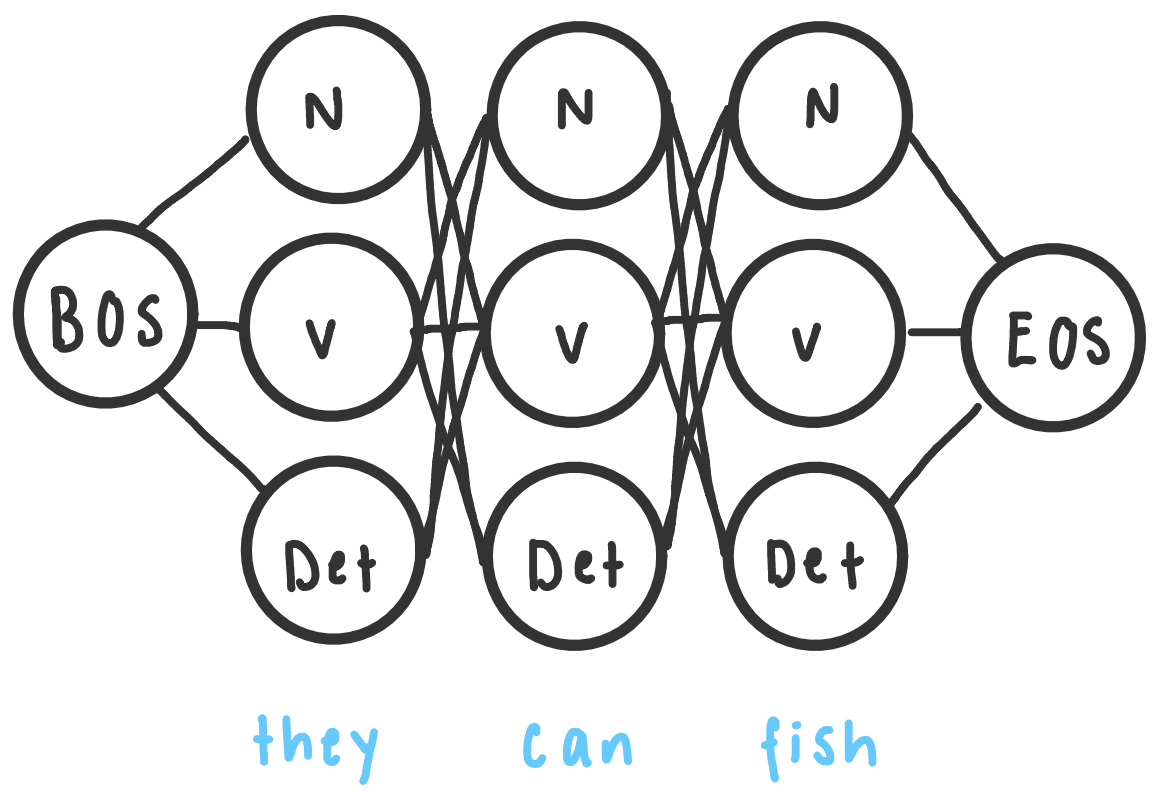
\includegraphics[height=10mm]{inhalt/images/NLP/06_pos_1.png}
\\\\
\textit{2) Backward algorithm}\\
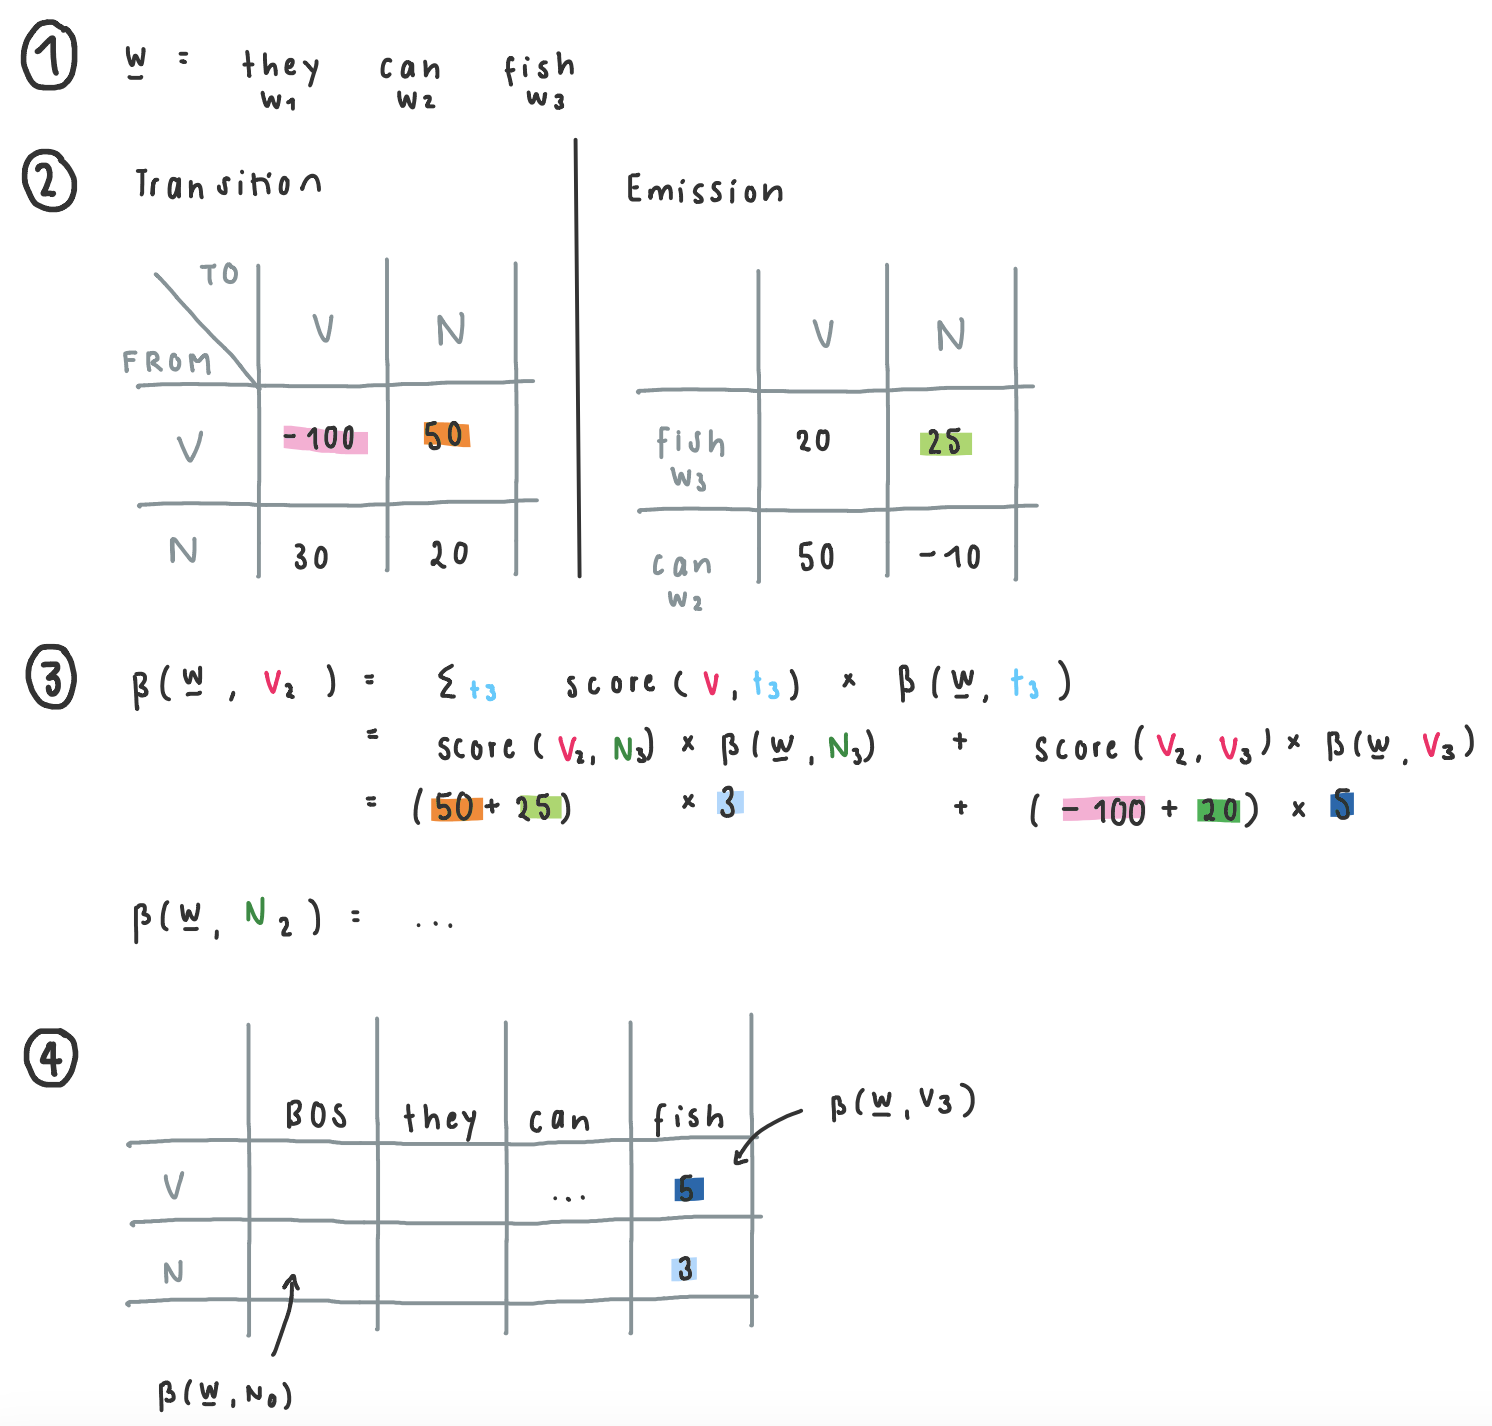
\includegraphics[height=25mm]{inhalt/images/NLP/06_pos_2.png}
\end{multicols}